\documentclass[11pt,a4paper,fontset=fandol]{ctexart}

\usepackage{geometry}
\geometry{a4paper, left=2.2cm, right=2.2cm, top=2.2cm, bottom=2.2cm, headheight=14pt}
\usepackage{setspace}
\linespread{1.05}
\usepackage{indentfirst}
\setlength{\parindent}{2em}
\emergencystretch=2em

\usepackage{xcolor}
\definecolor{themecolor}{RGB}{40,90,140}
\definecolor{codebg}{RGB}{248,248,245}

\usepackage{graphicx}
\graphicspath{{results/}}
\usepackage{amsmath}
\usepackage{booktabs}
\usepackage{caption}
\captionsetup{font=small,labelfont={bf,color=themecolor}}
\usepackage{subcaption}
\usepackage{float}
\usepackage{array}
\usepackage{verbatim}
\usepackage{hyperref}
\hypersetup{colorlinks=true, linkcolor=themecolor, citecolor=themecolor, urlcolor=themecolor!70!black}

\usepackage{titlesec}
\titleformat{\section}{\color{themecolor}\bfseries\fontsize{13}{16}\selectfont}{\thesection}{0.6em}{}
\titlespacing*{\section}{0pt}{0.9em}{0.35em}
\titleformat{\subsection}{\color{themecolor!85!black}\bfseries\fontsize{11.5}{14}\selectfont}{\thesubsection}{0.6em}{}
\titlespacing*{\subsection}{0pt}{0.55em}{0.15em}

\usepackage{fancyhdr}
\pagestyle{fancy}
\fancyhf{}
\renewcommand{\headrulewidth}{0.4pt}
\lhead{\small\color{black!55} 定位实验报告}
\rhead{\small\color{black!55} 人工智能 2302}
\cfoot{\small\color{black!55}\thepage}

\fancypagestyle{plain}{
  \fancyhf{}
  \renewcommand{\headrulewidth}{0pt}
  \cfoot{\small\color{black!55}\thepage}
}

\usepackage{mdframed}
\BeforeBeginEnvironment{verbatim}{
  \begin{mdframed}[
    backgroundcolor=codebg,
    linecolor=themecolor!30,
    linewidth=0.5pt,
    innerleftmargin=10pt,
    innerrightmargin=8pt,
    innertopmargin=6pt,
    innerbottommargin=4pt,
    skipabove=8pt,
    skipbelow=8pt,
    roundcorner=2pt,
  ]
}
\AfterEndEnvironment{verbatim}{\end{mdframed}}

\setCJKmonofont{Arial Unicode MS}

\title{\bfseries 定位实验报告}
\author{人工智能2302 \quad 蒋梓轩\\
人工智能2302 \quad 汪翌秦\\
人工智能2302 \quad 孙靖淞}
\date{2026 年 5 月 29 日}

\begin{document}

\maketitle

\section{实验目的}

本次实验在实验 3 已保存的静态地图基础上，启动 \verb|map_server|、RF2O 激光里程计和 AMCL 定位节点，实现机器人在已知地图中的全局重定位和连续位姿跟踪。实验通过 RViz 观察 \verb|map|、\verb|odom|、\verb|base_footprint| 的坐标变换关系，查看激光扫描、静态地图、机器人模型和粒子云分布是否匹配，从而验证定位链路是否正确。

实验重点包括：第一，理解 \verb|map -> odom -> base_footprint| 链式 TF 的意义；第二，理解 AMCL 如何利用粒子滤波在静态地图中估计机器人位姿；第三，理解 RF2O、轮式里程计、SLAM 和 AMCL 在 TF 发布中的分工；第四，观察参数和外界扰动对定位收敛性的影响。

\section{实验原理}

AMCL 是基于粒子滤波的蒙特卡洛定位方法。定位过程中，每个粒子代表一种可能的机器人位姿，运动模型根据里程计或激光里程计传播粒子，观测模型根据激光扫描与静态地图的匹配程度更新粒子权重。随着机器人运动和传感器观测不断输入，高权重粒子逐渐集中到真实位姿附近，RViz 中的 \verb|/particlecloud| 也会从分散状态逐渐收敛。

导航系统通常不直接发布 \verb|map -> base_footprint|，而是维护 \verb|map -> odom -> base_footprint|。其中 \verb|odom -> base_footprint| 连续、平滑，适合短时运动控制；\verb|map -> odom| 由定位算法修正，用于抵消里程计漂移。这样既保证底盘控制所需的局部连续性，又保证全局地图坐标下的位置准确性。

\begin{table}[H]
  \centering
  \caption{定位实验中的坐标系与节点分工}
  \begin{tabular}{lll}
    \toprule
    对象 & 主要作用 & 本实验来源 \\
    \midrule
    \verb|map| & 静态地图全局坐标系 & \verb|map_server| 加载 \verb|nav.yaml| \\
    \verb|odom| & 局部连续里程计坐标系 & RF2O 或底盘里程计 \\
    \verb|base_footprint| & 机器人底盘坐标系 & 机器人模型/底盘状态 \\
    \verb|map -> odom| & 全局定位修正 & AMCL \\
    \verb|odom -> base_footprint| & 局部运动估计 & RF2O 激光里程计 \\
    \bottomrule
  \end{tabular}
\end{table}

\section{实验步骤与结果分析}

\subsection{加载静态地图与定位节点}

实验首先将实验 3 保存的 \verb|nav.pgm| 与 \verb|nav.yaml| 放入 \verb|ebot_bringup/maps|，然后通过 \verb|test_amcl.launch| 启动地图服务、RF2O 和 AMCL：

\begin{verbatim}
roslaunch ebot_bringup test_amcl.launch
\end{verbatim}

其中 \verb|map_server| 负责发布 \verb|/map|；\verb|nav01_rf2o.launch| 启动激光里程计，发布 \verb|odom -> base_footprint|；\verb|nav01_amcl.launch| 加载 AMCL 参数，发布 \verb|map -> odom|。三个模块组合后形成完整的定位 TF 链。

\begin{verbatim}
<node name="map_server" pkg="map_server"
      type="map_server" args="$(find ebot_bringup)/maps/nav.yaml"/>
<include file="$(find ebot_bringup)/launch/nav01_rf2o.launch"/>
<include file="$(find ebot_bringup)/launch/nav01_amcl.launch"/>
\end{verbatim}

\subsection{静态地图与初始位姿校准}

AMCL 的前提是当前激光扫描能够与静态地图在同一坐标体系下对齐。实验中使用的地图来自实验 3 保存的 \verb|nav.yaml| 和 \verb|nav.pgm|，地图分辨率为 \verb|0.05 m/cell|。启动 RViz 后，先将 Fixed Frame 设置为 \verb|map|，再添加 Map、LaserScan、TF 和 PoseArray。若初始粒子云与真实位置偏差较大，则使用工具栏中的 \verb|2D Pose Estimate| 在地图上给出机器人初始位姿，使粒子云快速收敛到障碍物边界匹配的位置。

\begin{figure}[H]
  \centering
  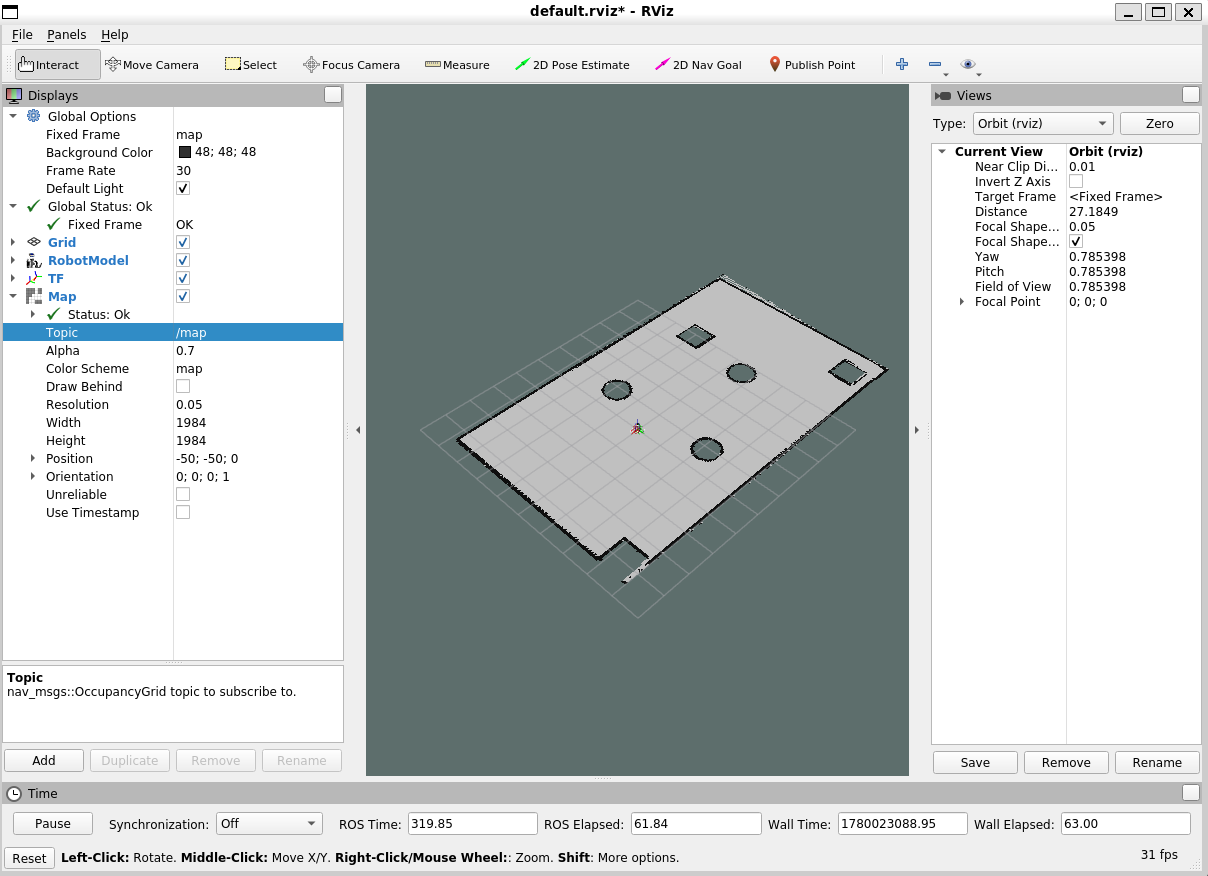
\includegraphics[width=0.72\linewidth]{lab3_rviz_map.png}
  \caption{实验 4 使用的实验 3 静态地图。}
  \label{fig:lab4-map}
\end{figure}

\subsection{RViz 可视化定位结果}

在 RViz 中添加 Map、LaserScan、TF、RobotModel 和 PoseArray 显示项后，可以同时观察静态地图、雷达扫描点、机器人坐标系和粒子云。图 \ref{fig:lab4-amcl} 显示机器人位姿已经叠加到静态地图上，激光扫描与障碍物边界基本吻合，说明 AMCL 对机器人在地图中的位置估计是有效的。

\begin{figure}[H]
  \centering
  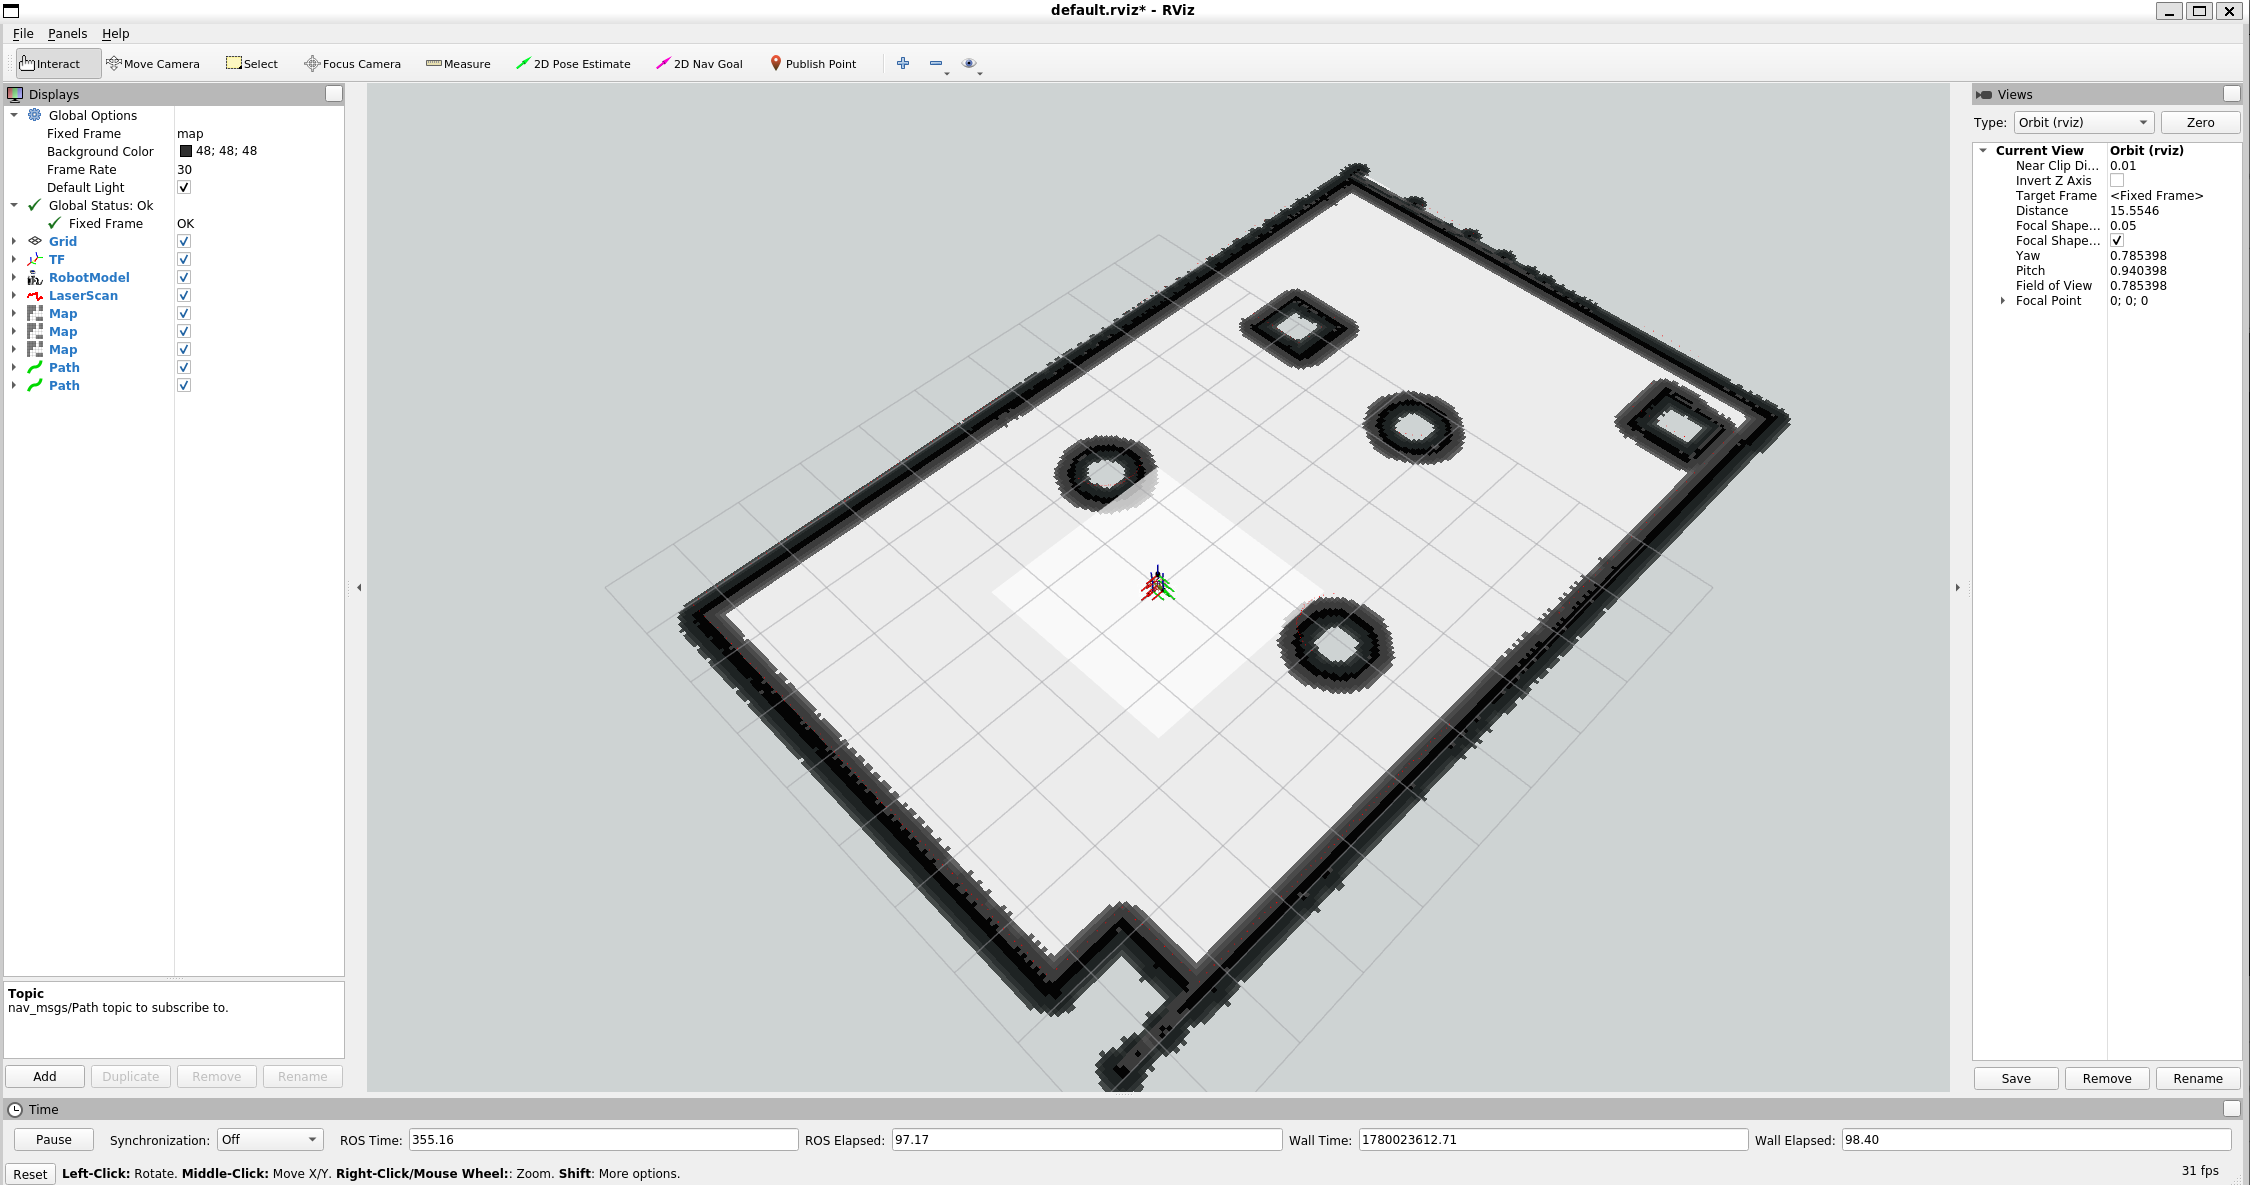
\includegraphics[width=0.95\linewidth]{lab4_amcl.png}
  \caption{实验 4 静态地图中的 AMCL 定位显示。}
  \label{fig:lab4-amcl}
\end{figure}

\subsection{参数与鲁棒性分析}

AMCL 的定位效果与粒子数量、运动更新阈值和观测模型参数密切相关。本实验配置中 \verb|min_particles| 为 500，\verb|max_particles| 为 5000，能够在重定位阶段保留较多候选位姿；\verb|update_min_d| 和 \verb|update_min_a| 控制机器人移动多少距离或转动多少角度后触发更新，阈值过大会导致粒子云更新滞后，阈值过小则会增加计算开销。

当短时遮挡激光雷达或人为改变机器人位姿时，粒子云会出现扩散或偏移。如果机器人继续运动并重新获得稳定扫描，AMCL 可以依靠静态地图匹配逐步恢复；如果初始位姿偏差过大，则需要通过 RViz 的 \verb|2D Pose Estimate| 手动给出更接近真实位置的初值。

\begin{table}[H]
  \centering
  \caption{AMCL 关键参数与影响}
  \begin{tabular}{lll}
    \toprule
    参数 & 本实验取值 & 影响 \\
    \midrule
    \verb|min_particles| & 500 & 粒子数下限，影响稳定跟踪计算量 \\
    \verb|max_particles| & 5000 & 粒子数上限，影响全局重定位能力 \\
    \verb|laser_model_type| & \verb|likelihood_field| & 使用似然场模型匹配激光与地图 \\
    \verb|update_min_d| & 0.2 & 平移更新阈值，过大时更新滞后 \\
    \verb|update_min_a| & 0.5 & 角度更新阈值，影响转弯时粒子更新 \\
    \verb|transform_tolerance| & 0.1 & TF 查询容忍时间，过小可能导致外推错误 \\
    \bottomrule
  \end{tabular}
\end{table}

\subsection{定位效果判断}

定位是否成功不能只看机器人图标是否显示在地图中，还要同时检查三类证据。第一，LaserScan 点云应与地图中墙体或障碍物边界重合，如果整体平移或旋转，说明初始位姿或 TF 可能有误；第二，PoseArray 粒子云应从分散逐渐收敛，若粒子长时间分散，说明观测模型难以区分当前位置或传感器数据不稳定；第三，TF 树应保持 \verb|map -> odom -> base_footprint -> laser_frame| 连通，若缺少某一段，RViz 可能无法把激光数据投影到地图坐标系。

实验截图中，静态地图、激光扫描和机器人模型能够同时显示，说明地图、雷达和底盘坐标已经被统一到 \verb|map| 坐标系下。机器人移动时，\verb|odom -> base_footprint| 提供平滑短期运动，AMCL 根据扫描匹配持续修正 \verb|map -> odom|，因此机器人在全局地图中的位置不会因里程计累计误差无限漂移。

\newpage
\section{结论与问题讨论}

本实验完成了静态地图加载、RF2O 里程计发布、AMCL 定位和 RViz 可视化验证。实验结果表明，机器人在已有地图中能够形成完整的 \verb|map -> odom -> base_footprint| 坐标链，激光扫描与地图障碍物边界吻合，定位结果可供后续 \verb|move_base| 路径规划使用。

\textbf{map、odom、base\_footprint 的含义。}
\verb|map| 是全局静态地图坐标系，允许定位算法进行跳变式全局修正；\verb|odom| 是局部连续坐标系，短时间内平滑但长期会漂移；\verb|base_footprint| 是机器人底盘投影坐标系，表示机器人当前运动主体。

\textbf{为什么使用 map -> odom -> base\_footprint。}
如果 AMCL 直接发布 \verb|map -> base_footprint|，定位修正会直接作用到底盘位姿，容易造成控制链路中的位姿跳变。链式结构把全局修正放在 \verb|map -> odom|，把连续运动放在 \verb|odom -> base_footprint|，兼顾全局准确性和局部连续性。

\textbf{不同算法负责的 TF 段。}
轮式里程计或 RF2O 通常发布 \verb|odom -> base_footprint|；AMCL 在静态地图上发布 \verb|map -> odom|；Gmapping 等 SLAM 算法在建图时估计机器人相对于地图的位置，并发布或维护 \verb|map| 与里程计链之间的关系；Hector 更依赖激光匹配，可在里程计较弱时提供位姿估计。

\textbf{RF2O 与 Gmapping 能否结合实车建图。}
可以结合，但前提是 TF 和话题配置正确：先启动底盘、雷达和静态 TF，再启动 RF2O 发布 \verb|odom -> base_footprint|，最后启动 \verb|gmapping| 订阅 \verb|/scan| 并使用该里程计链建图。若雷达帧、底盘帧或时间戳不一致，地图会出现漂移、重影或无法更新。

\textbf{不同分辨率地图对定位的影响。}
分辨率较高的地图能保留更多墙体和障碍物细节，激光匹配时特征更丰富，但地图文件更大、匹配计算量也更高；分辨率较低的地图更平滑，噪声少、计算快，但狭窄区域和小障碍物可能被模糊，导致粒子权重区分度下降。实验中采用 \verb|0.05 m/cell| 作为折中配置，能够兼顾定位精度和实时性。

\textbf{定位异常时的处理。}
如果机器人在 RViz 中出现明显跳变或粒子云持续发散，应先检查 \verb|/scan| 是否正常、TF 是否连通、地图原点和分辨率是否正确；再用 \verb|2D Pose Estimate| 重新给定初始位姿；最后再考虑调整粒子数量、运动噪声和激光模型参数。这样可以把“配置错误”和“参数不佳”分开排查。

\end{document}
